\section{$Re_{\tau}=1000$ simulation} 
The second simulation performed is carried out at $Re_{\tau}=1000$, which in terms of channel width and bulk velocity is equivalent to $Re_{b}=40000$.\par
Such velocity, obtained as shown in the previous chapter, is 19.79, while $\alpha_{0}$ and $\beta_{0}$ are respectively 0.5 and 1, for the reasons shown before.\par
The timestep is once again constant, with \emph{dt}=0.0005 and the simulation time is T=5. \par
The simulation time is smaller than before for costing reasons, however, in order to guarantee good results, we sampled the field every 0.05 steps, so that we can employ a 100 fields to do the ensemble average.\\~\par
The grid employed in this simulation face 500 points in the wall-normal direction, 2048 in the spanwise direction and 2048 points along the streamwise dimension, direction in which we exploit the Hermitian symmetry. According to this configuration, the grid size reach the billion of points.\par
Table~\ref{table:1000} report a summary of the simulation configuration for the $Re_{\tau}=1000$ case.\\~\par

\begin{table}
\caption{Simulation data for $Re_{\tau}$=1000}
\begin{center}
\begin{tabular}{ccccccccccccc}
\toprule
$L_{x}$ & $L_{z}$ & $\delta$ & $nx$ & $nz$ & $ny$ & $\alpha_{0}$ & $\beta_{0}$ & $\Delta x^{+}$ & $\Delta z^{+}$ & $px$ & $dt$ & $T$\\
$4\pi$ & $2\pi$ & 1 & 2048 & 2048 & 500 & 0.5 & 1 & 6.1  & 3 & 1 & 0.0005 & 5 \\
\bottomrule
\end{tabular}
\end{center}
\label{table:1000}
\end{table}


Since are required approximately 40GB of disk space per each field we decided to avoid to save on disk them, instead we calculated the statistics runtime, merging the files at the end of the simulation, reducing the required space to few MB.\\~\par

Let us focus now on the statistics gained from the simulation.\par
Figure~\ref{loglaw:1000} report the law of the wall. As we can see from the plot, made in semi-logarithmic scale using the wall units, our result fits the expected curve.\par
Far from the wall, the velocity defect law find good feedback with our results, as shown by the graph~\ref{velocity:defect:1000}.\\~\par

\begin{figure}
\begin{center}
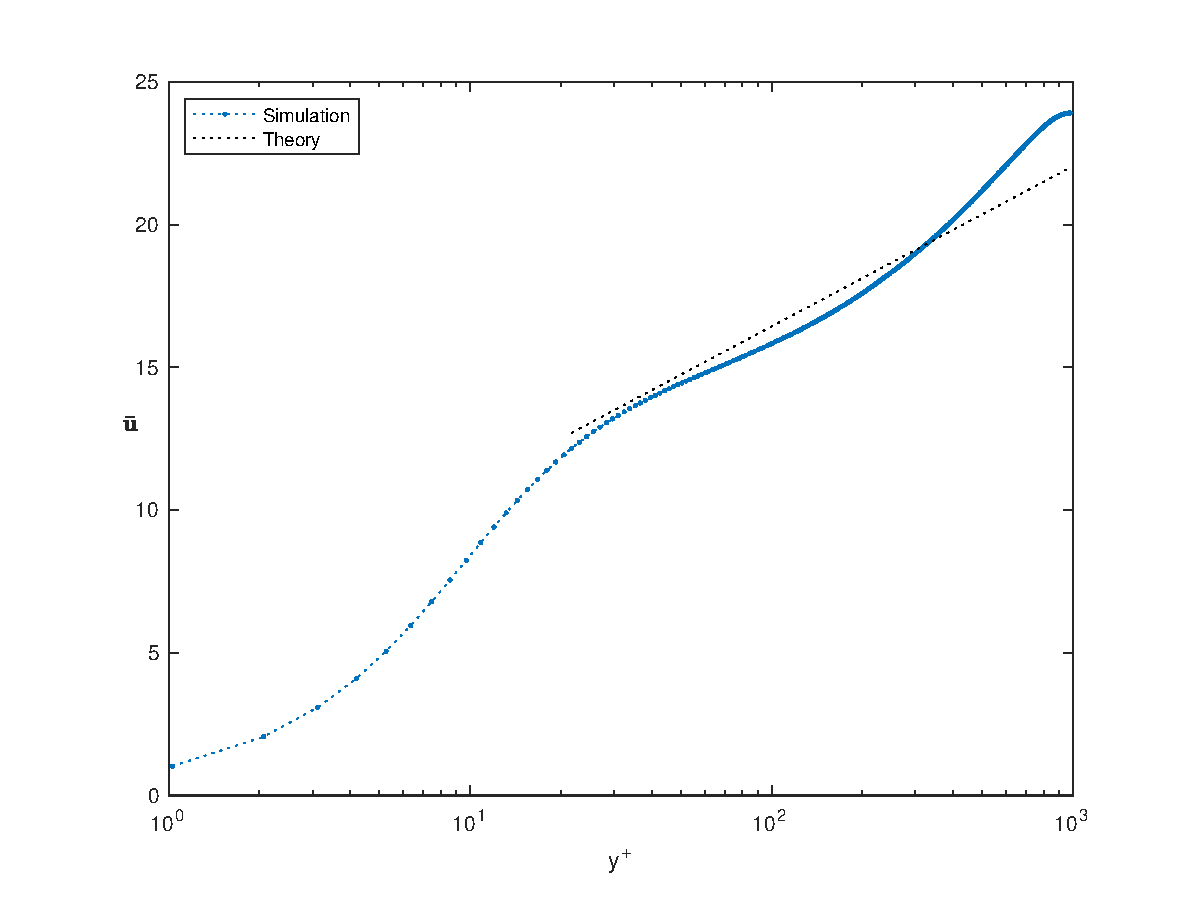
\includegraphics[scale=0.55]{grafici/loglaw_1000.eps}
\caption{$\bar{u}^{+}$ in the near wall region for a $Re_{\tau}=1000$ simulation}
\label{loglaw:1000}
\end{center} 
\end{figure}

\begin{figure}
\begin{center}
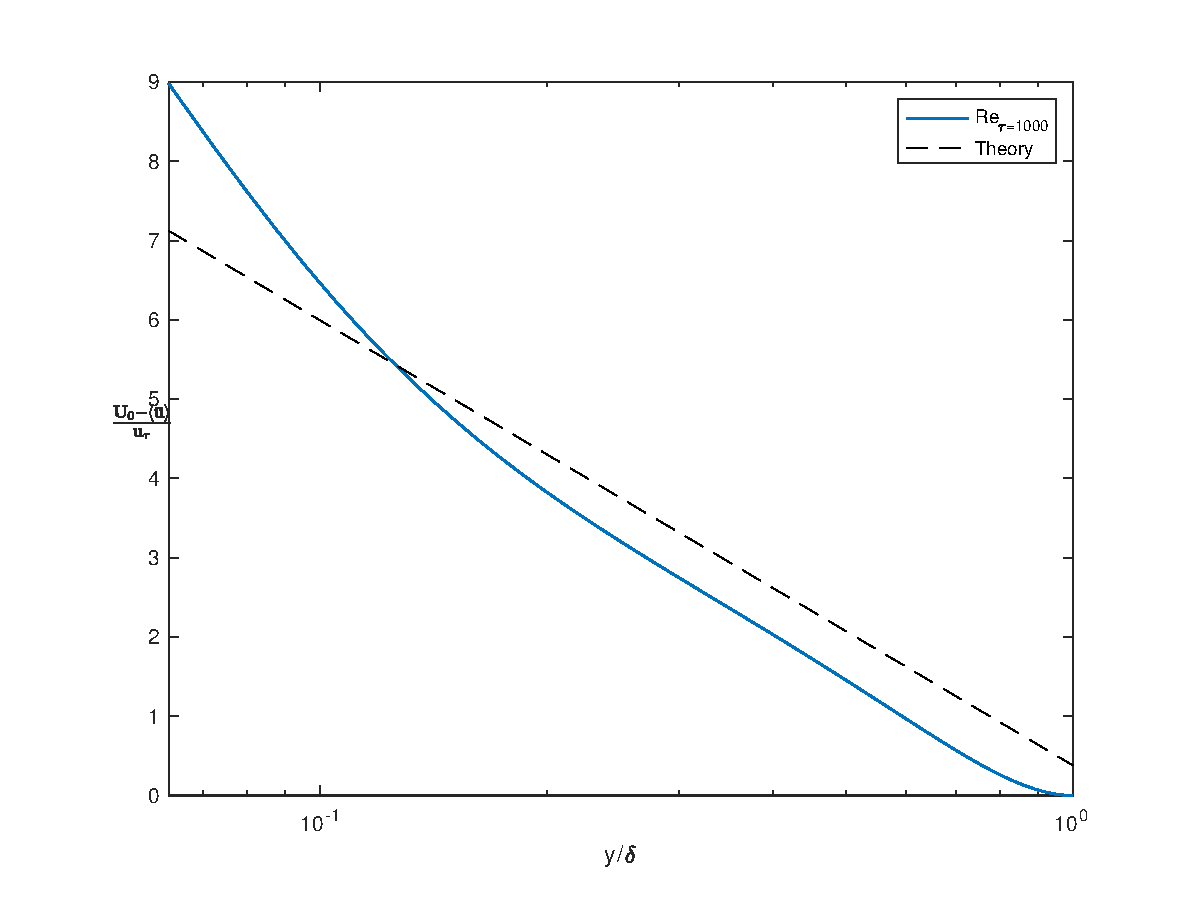
\includegraphics[scale=0.55]{grafici/velocity_defect_1000.eps}
\caption{Velocity defect for a $Re_{\tau}=1000$ simulation}
\label{velocity:defect:1000}
\end{center} 
\end{figure}

In figure~\ref{budget:1000} we reported the \emph{rms} fluctuations, normalized by the $u_{\tau}^{2}$, jointed with the TKE distribution. The first differences that we can immediately face by comparing our curves with the ones in figure~\ref{k+budgets:180} are the peak values. These values tends to increase with respect to the counterpart of the $Re_{\tau}=180$ simulation, highlighting how this simulation contains more energy than the previous ones.\par
Although the \emph{rms} face higher peak values, their curves shapes tends to remain aligned with the ones seen during the previous simulation, at exception of the spanwise fluctuations which, instead, tends to become more sharpened in the near wall region. Such behavior can be linked to an higher turbulence presence.\\~\par
Finally I would like to briefly analyze the shape of the turbulent kinetic energy. Such curves cross $uu^{+}/u_{\tau}$ around the 50 wall units and exhibit a more sloped profile with respect to the $Re_{\tau}=180$ simulation. Despite of this latter condition, the value at the centerline does not exhibit changes across the two simulations.\\~\par

\begin{figure}
\begin{center}
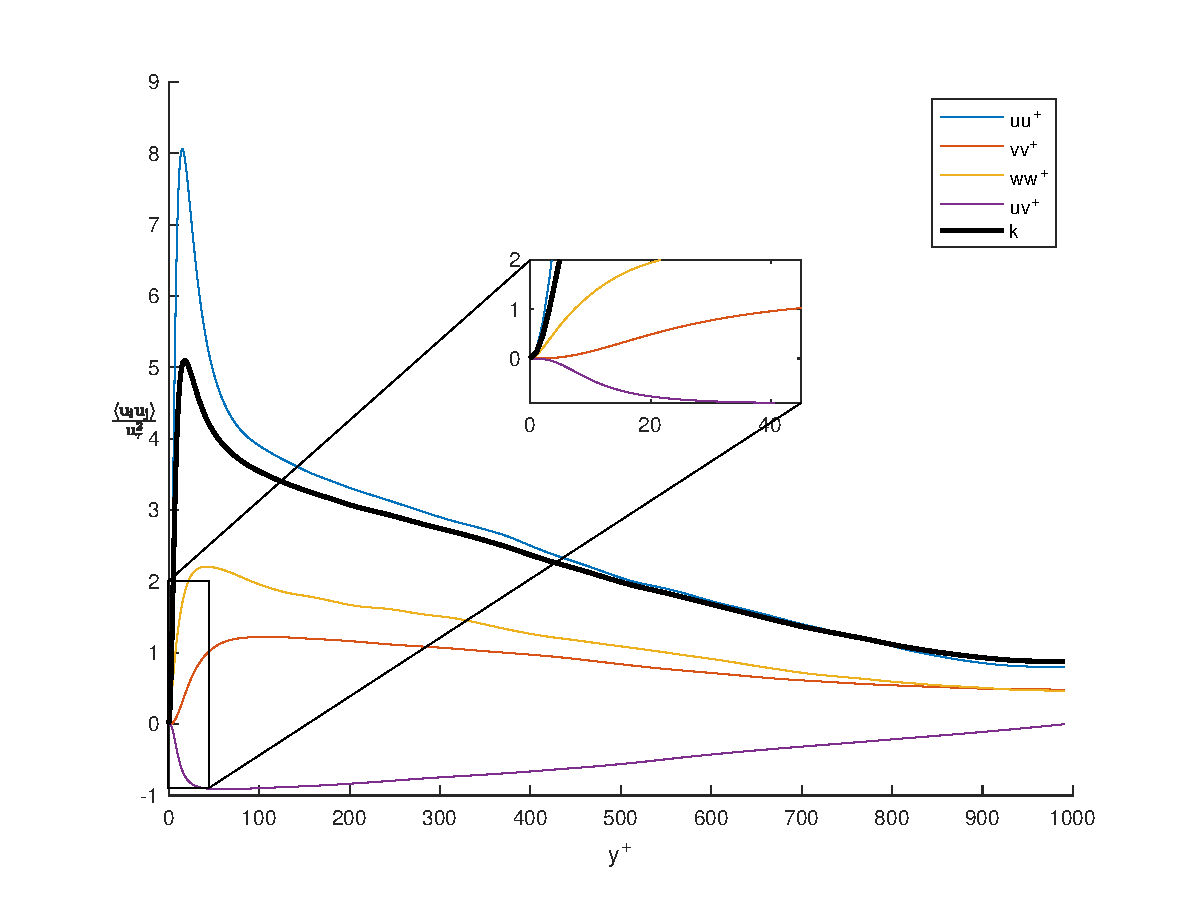
\includegraphics[scale=0.55]{grafici/budget+k_1000.eps}
\caption{\emph{rms} terms for a $Re_{\tau}=1000$ simulation}
\label{budget:1000}
\end{center} 
\end{figure}


The finer mesh and the higher Reynolds evidenced the appearance of a new turbulence peak, detached from the wall-cycle, identified by knees in the curves represented in figure~\ref{rms:1000}. Although the profiles are similar, with exception for the higher peaks reached, in the near wall region, they behave differently moving towards the inner region of the flow. In particular, by looking at $u'/u_{\tau}$, the sketchy knee present around $y^{+}\approx 100$ in figure~\ref{rms:kmm:180} now results to be fully developed and has moved towards the centerline, approximately around $y^{+}\approx 400$. The peak does not differ too much in the two simulations, with values of $2.6\sim2.7$ located at $y^{+}\approx14$, however, the higher energy content manifest through the trailing values. These terms shows an upward bias, if compared with the $Re_{\tau}=180$ values, plus the presence of the already cited knee.\par
Similar behavior is expressed by $w'/u_{\tau}$, although in its case the increase in terms of peak value is consistent, with a slightly decrease of the peak coordinate towards $y^{+}\approx30$. Also in this case the appearance of the knee is approximately around $y\approx 400$.\par
Also the term $v'/u_{\tau}$ face a huge increment of the peak value, in first approximation we may say that it doubles its value with respect to $Re_{\tau}=180$ simulation. In such case identifying the knee is less straightforward. However, we can observe that the area under the curve has clearly increased.\\~\par

\begin{figure}
\begin{center}
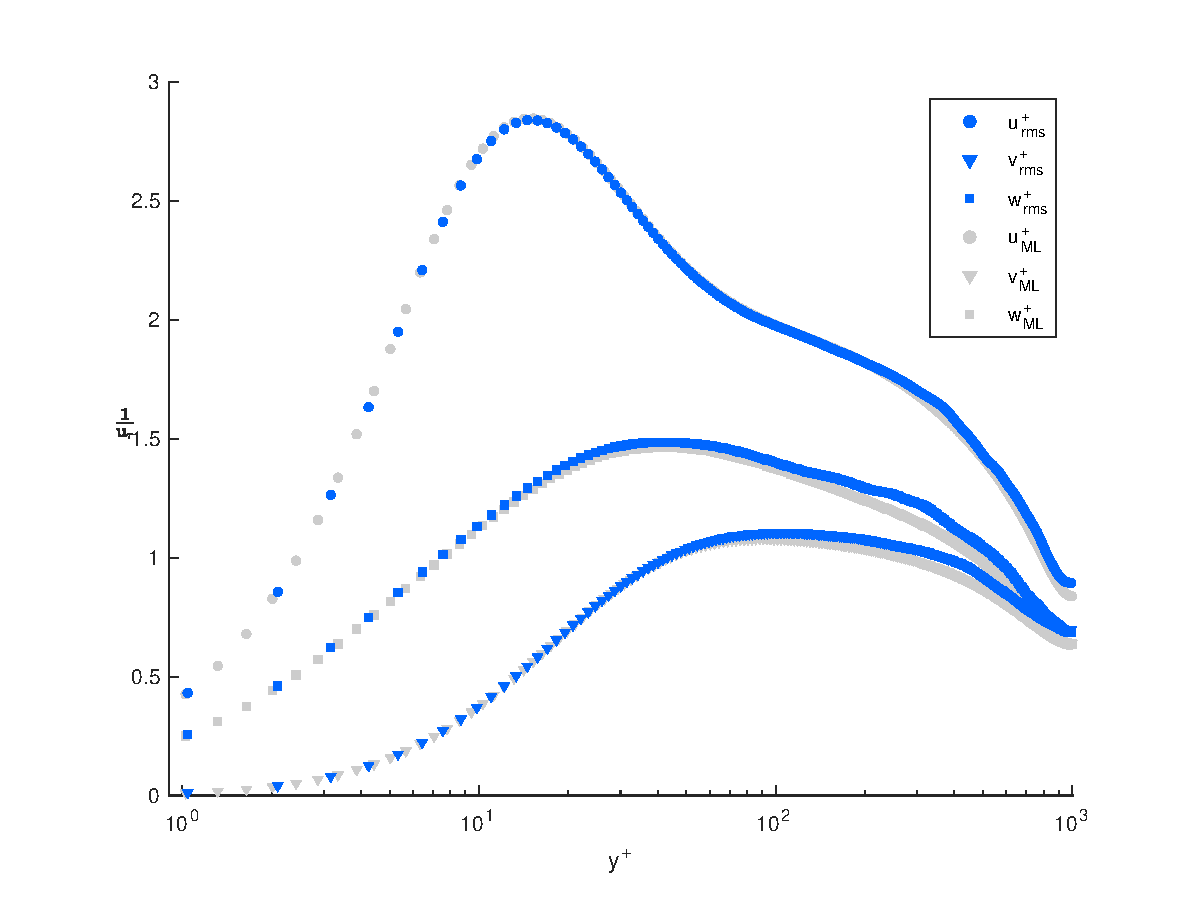
\includegraphics[scale=0.55]{grafici/rms_1000.eps}
\caption{\emph{rms} behavior on a $Re_{\tau}=1000$ simulation}
\label{rms:1000}
\end{center} 
\end{figure}

\begin{figure}
\begin{center}
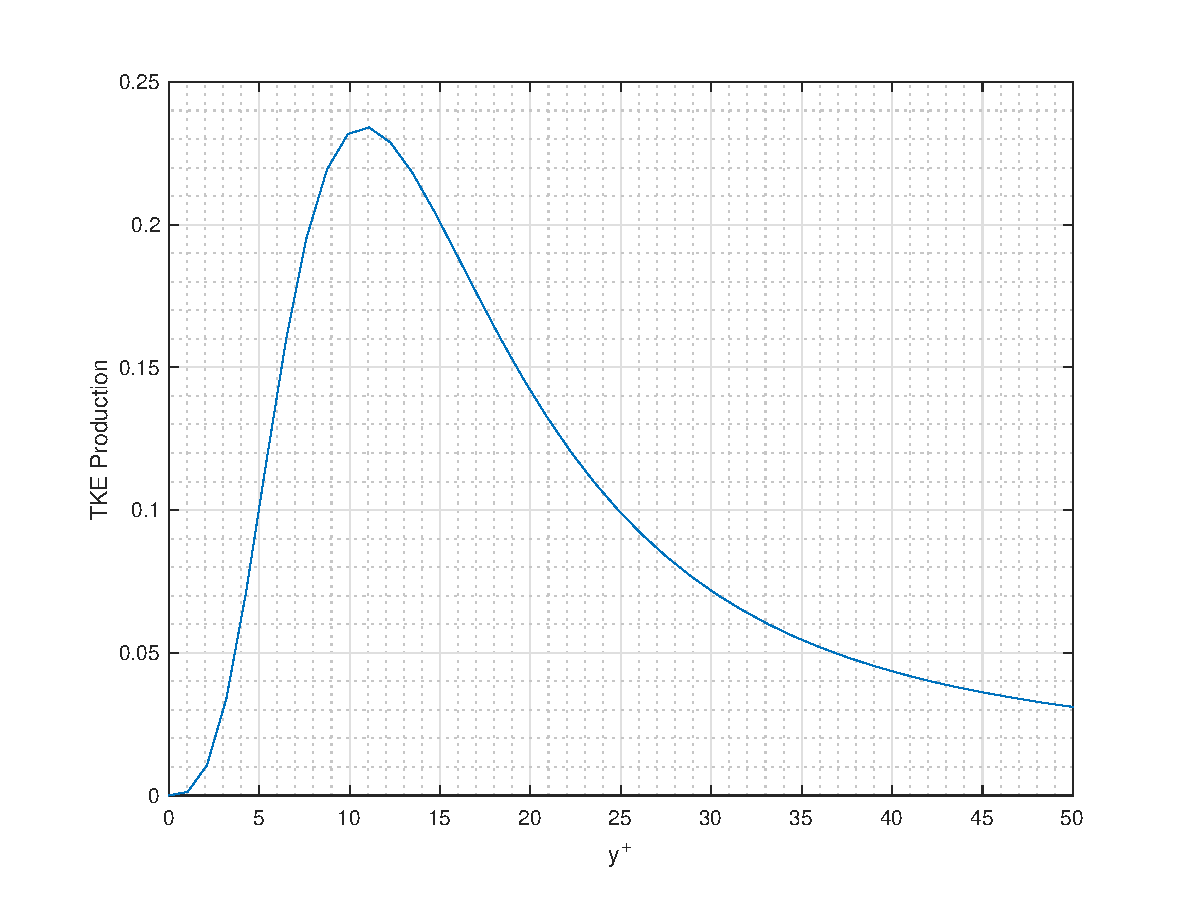
\includegraphics[scale=0.55]{grafici/tke_prod_1000.eps}
\caption{Production term of the TKE eq. for a $Re_{\tau}=1000$ simulation}
\label{tke:prod:1000}
\end{center} 
\end{figure}

The \emph{rms} terms near the wall does not exhibit marked changes, the same applies also for the graphs of the \emph{production}, reported in figure~\ref{tke:prod:1000}, that reach a slightly higher peak of $P/Re_{\tau}=0.24$, located at $y\approx12$.\\~\par

As theory affirms, the wall coordinate of the peak of production corresponds to that in which the stress components become equivalent. This aspect will be detailed further, comparing the results of all the simulations together.
At the present we limit to present the behavior of the stress components, which is reported in figure~\ref{stresses:1000}.

\begin{figure}
\begin{center}
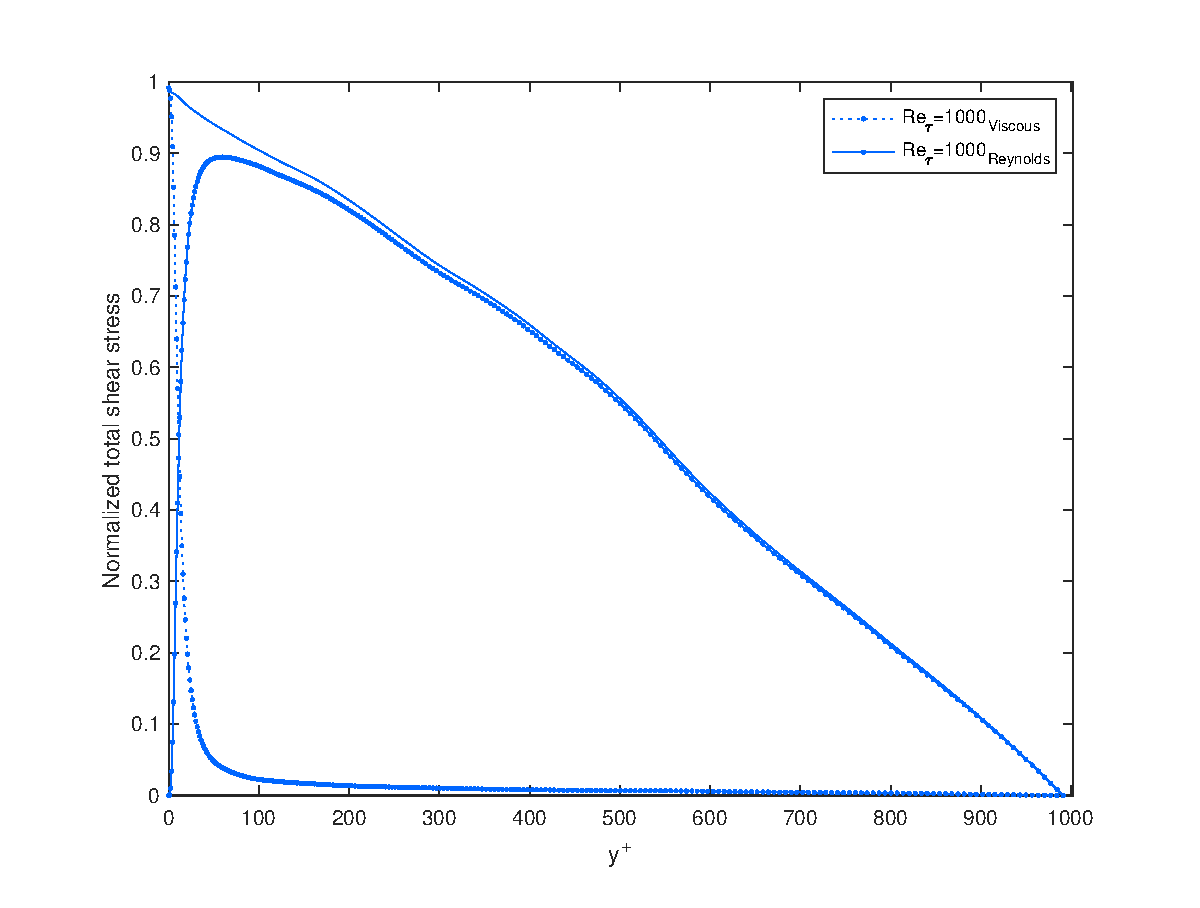
\includegraphics[scale=0.55]{grafici/stresses_1000.eps}
\caption{Normalized total shear stress for a $Re_{\tau}=1000$ simulation}
\label{stresses:1000}
\end{center} 
\end{figure}